Machine learning is a subfield of artificial intelligence, `concerned with the question of how to construct computer programs that automatically improve with experience.' \cite{Mitchell97}
Supervised machine learning is one of the three machine learning disciplines, besides unsupervised and reinforcement learning.
The goal is to find a mapping between an input and an output, in our case an excitation and its respective optimal harvesting policy.
Multiple algorithms to find such a mapping exist, however for high dimensional problems artificial neural networks (ANNs) are usually used.
In the following sections we review two ANN architectures, the fully-connected feedforward ANN and the Long Short-Term Memory (LSTM) network.

\subsection{Fully-connected feedforward ANNs}
In this section we review ANNs, following the exposition given in \cite{lu2020dying}.

Let $\textfrak{N}$ be a fully-connected feedforward ANN, meaning there are no loops in the neuron connections and all neurons in a layer are connected to every neuron of the next layer, $\textfrak{N}: \mathbb{R}^{n_1} \to \mathbb{R}^{n_L}$. $n_1$ and $n_L$ denote the dimensionality of the input and output respectively. 
$\textfrak{N}$ has $L$ layers, or columns of neurons.
The network architecture is given by the amount of neurons $n_l$ in each hidden layer $l \in [2, L - 1]$ (see figure \ref{nn}).
The neurons in layer $l$ are represented by their activations $\vec{a}_l \in \mathbb{R}^{n_l}$, which represent the matrix multiplication output. Additionally each layer includes trainable parameters $W_l \in \mathbb{R}^{n_{l+1} \times n_{l}}$ and $\vec{b}_l \in \mathbb{R}^{n_l}$ called weights and biases.
The activations can then be calculated using the following formulae \cite{TN_libero_mab2)53517}:
\begin{align*}
	\vec{a}_2 & = W_1 \vec{a}_1 + \vec{b}_1, \\
	\vec{a}_l & = W_{l-1} \xi(\vec{a}_{l-1}) + \vec{b}_{l-1}, \ l \in [3, L],
\end{align*}
where $\xi(x)$ is a function called the activation function applied elementwise. Historically, functions such as $tanh$ and sigmoid have been used. However, it has been shown \cite{Maas2013RectifierNI, krizhevsky} that the rectified linear unit $\mathrm{ReLU}(x) = \mathrm{max}(0, x)$ often provides better results and is used here.


\subsection{Long Short-Term Memory}
While the network architecture introduced in the previous section performs reasonably well on many problems, it destroys 

To train an ANN a cost function is defined, often the mean squared error 
\begin{align*}
	\mathrm{MSE} = \frac{1}{N} \sum_{i=1}^N (\vec{a}_{L, i} - \vec{y}_i)^2,
\end{align*}
where the summation is performed over the training data $\{(\vec{x}_i, \vec{y}_i)\}$ with $N$ samples, where $\{\vec{x_i}\}$ is the input and $\{\vec{y_i}\}$ the output data, and $\vec{a}_{L, i} = \textfrak{N}(\vec{x}_i)$ is the output of the neural network.
The so-called backpropagation algorithm is used to calculate the gradient of the cost function with respect to the trainable parameters and improve the performance of the ANN \cite{rumelhart1986learning, nielsenneural}.

\begin{figure}
	\centering
	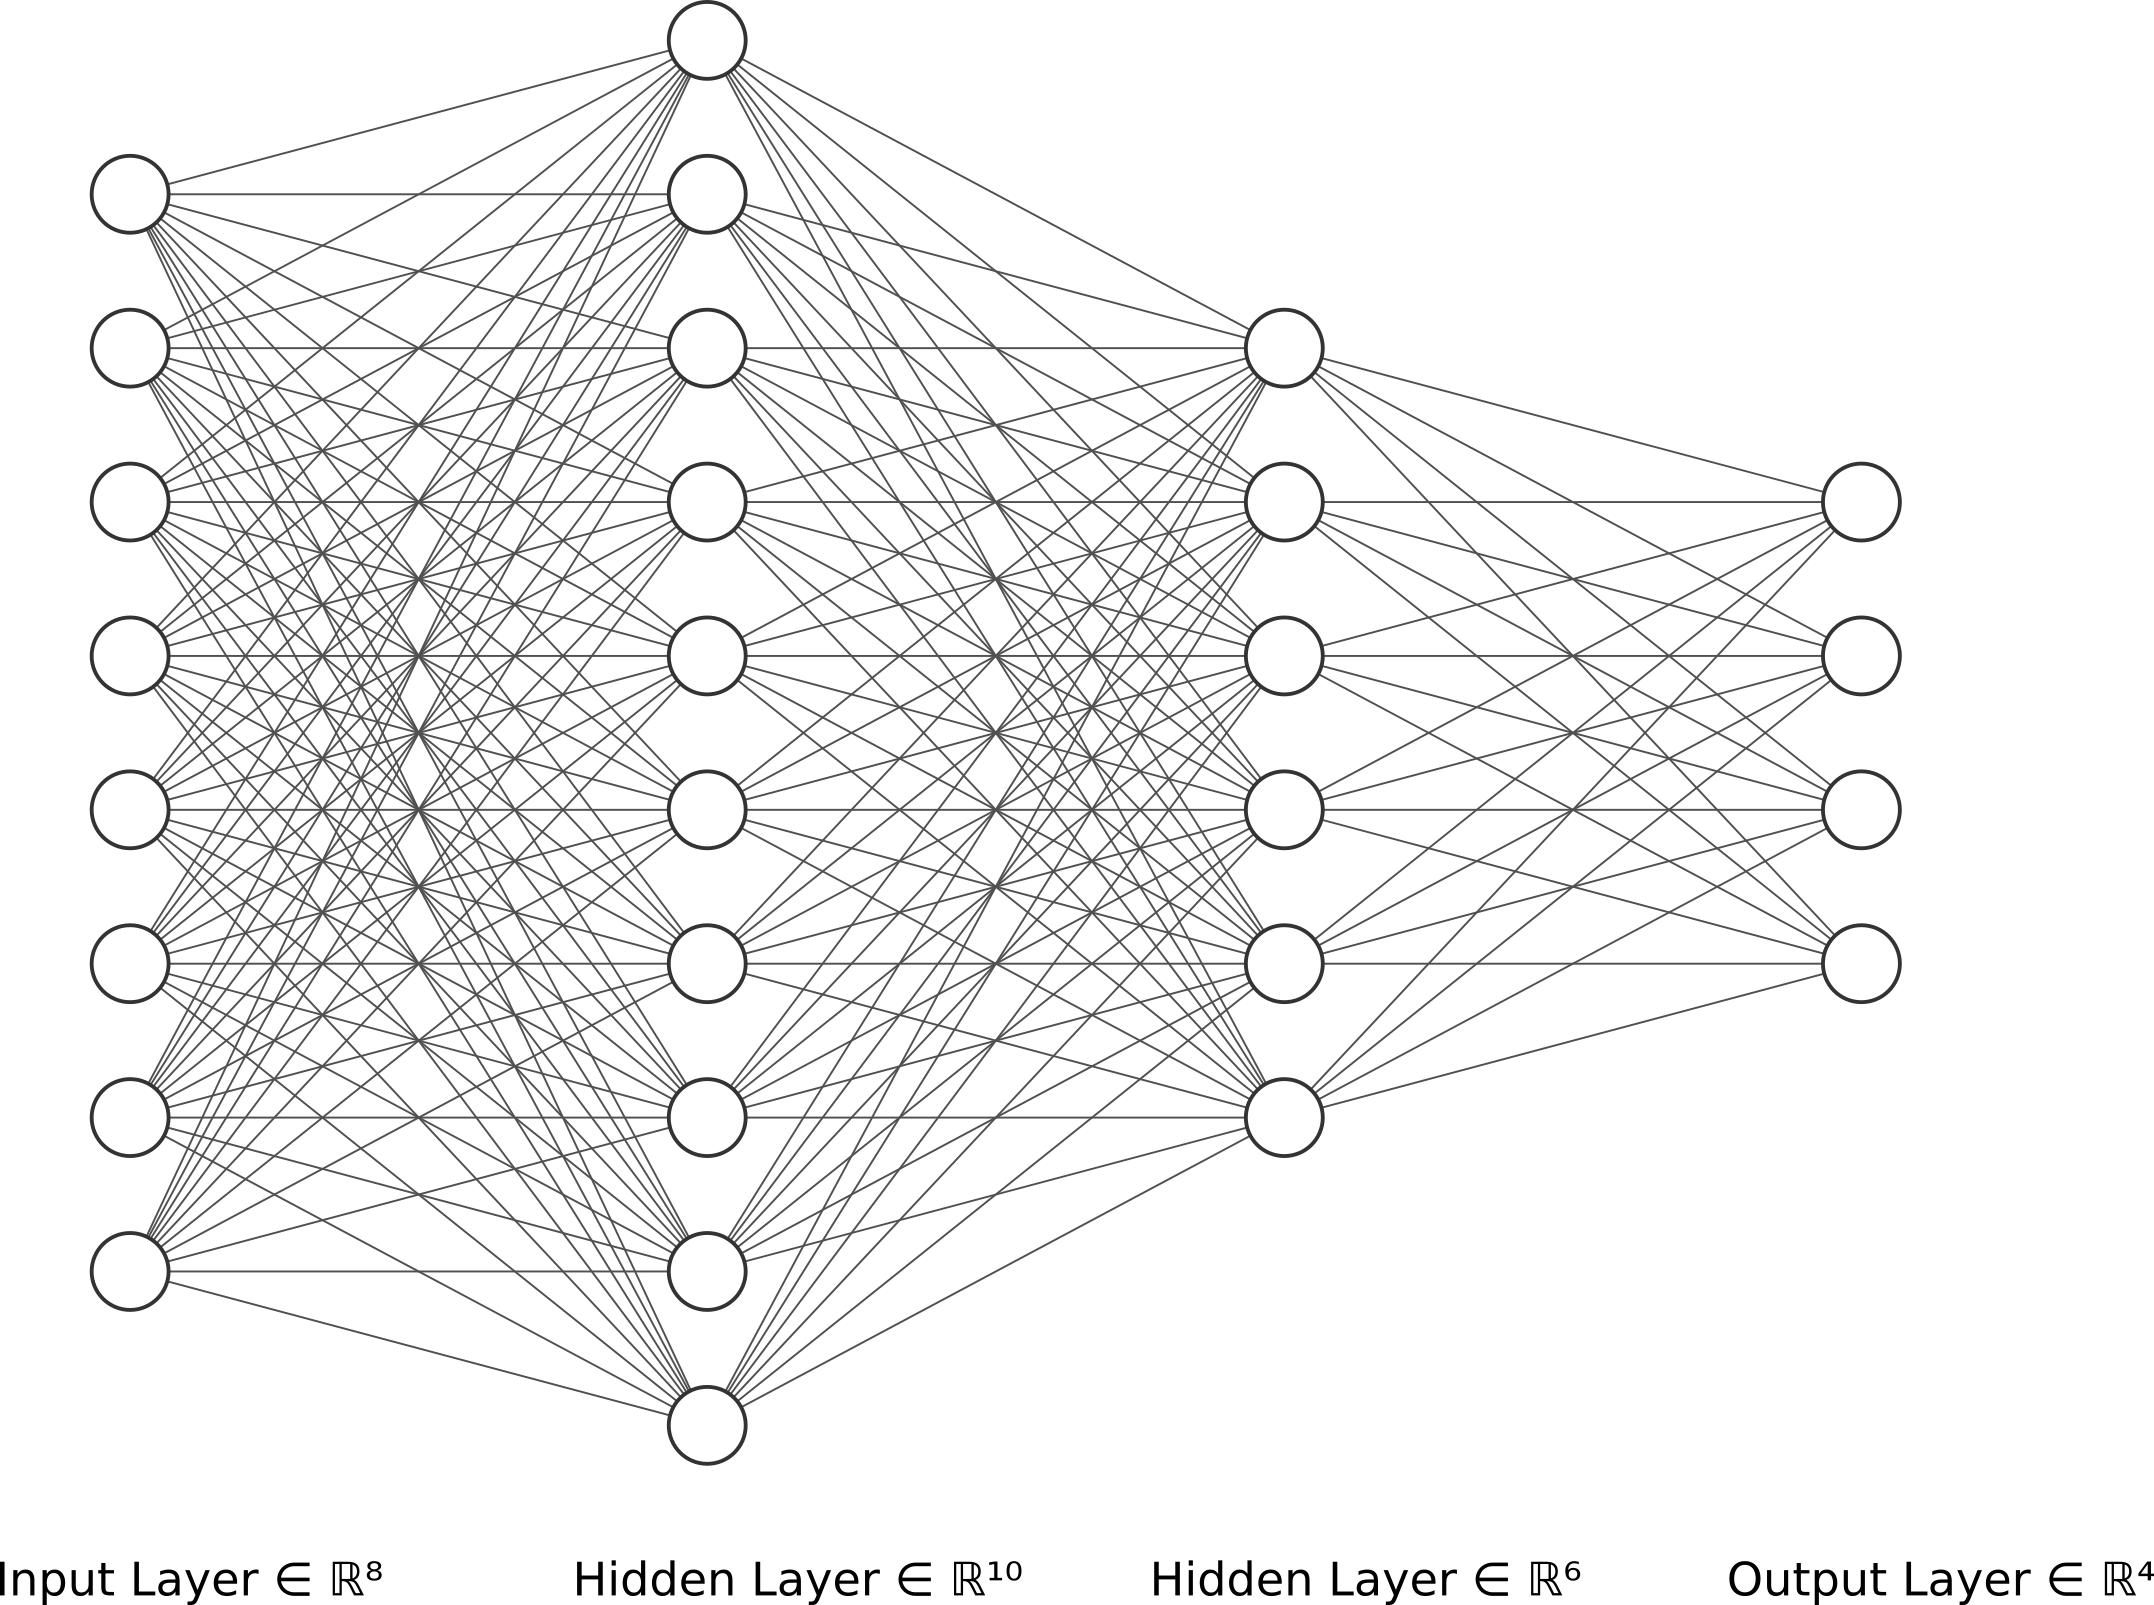
\includegraphics[width=0.6\textwidth]{img/nn}
	\caption{Example fully-connected feedforward ANN with four layers, including input, output and two hidden layers \cite{LeNail2019}}.
	\label{nn}
\end{figure}